\begin{figure}[H]
	    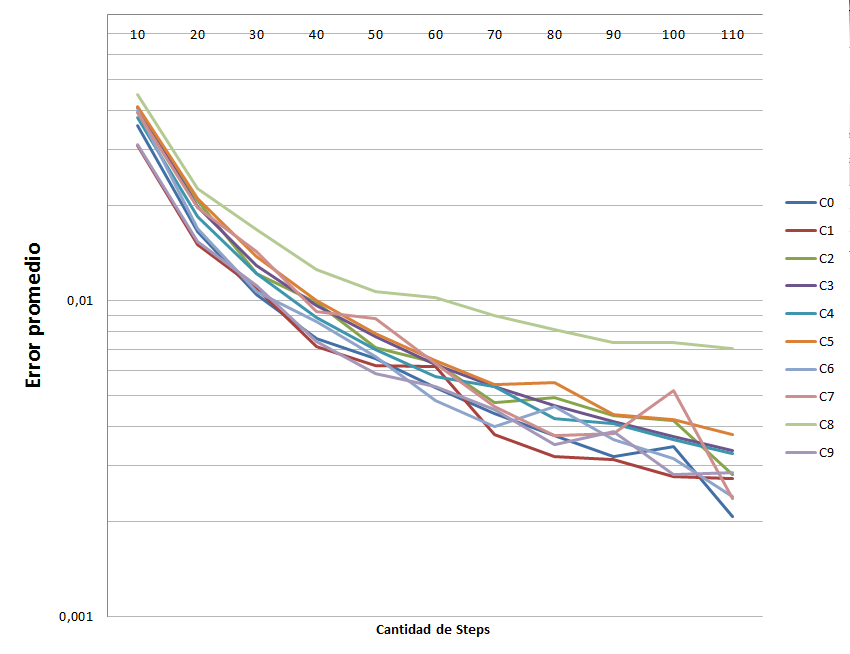
\includegraphics[scale=.60]{imagenes/variacion_parametro_y_columna_steps.png}
	    \caption{Error promedio en Steps para todas las columnas de la tabla brindada por la materia} 
	    \label{fig:variacion_parametro_y_columna_steps}
\end{figure}

	A continuaci\'on, realizamos un an\'alisis del estimador ``Distributed Steps'', el cual obtuvo los mejores resultados seg\'un nuestros an\'alisis previos.
	
	En la figura \ref{fig:variacion_parametro_y_columna_steps} se ve un gr\'afico que se realizo utilizando los errores promedio para cada columna, variando a la ves la cantidad de Steps del estimador y estimando por igualdad. Como error promedio consideramos al promedio de los errores obtenidos para los distintas estimaciones de los valores de una misma columna. Una ves teniendo el error promedio para una cantidad de Steps particular y una columna particular, repetimos el proceso variando la cantidad de Steps para todas las columnas.
	
	Se ve como el error promedio de cada columna, en si es muy similar para pocos Steps, pero al aumentar la cantidad de steps, mejora mucho el error, y esta mejora es bastante independiente de la distribuci\'on de la columna, ya que la diferencia de errores entre columnas, es muy chico.

	Solo para la columna C8 se ve como el error es considerablemente mayor al resto. Esta columna es particularmente distinta a las dem\'as, ya que sus datos van de 0 a 41 y son de una distribuci\'on que no es ni normal ni uniforme, sino que es mas bien como una ``media campana'' con media en el 0, y que va disminuyendo a medida que se acerca al 41, en donde pasa a ser 0. En la archivo ``/tests/Determinar Distribuciones/c8\_distro.xlsx'' se puede ver el gr\'afico del mismo. Sin embargo, por mas de que en esta columna el error haya subido un poco, sigue estando en un valor bastante bajo, por lo que se puede concluir que ``Distributed Steps'' la distribuci\'on de los datos no influye demasiado en el error.
	
	
\begin{figure}[H]
	    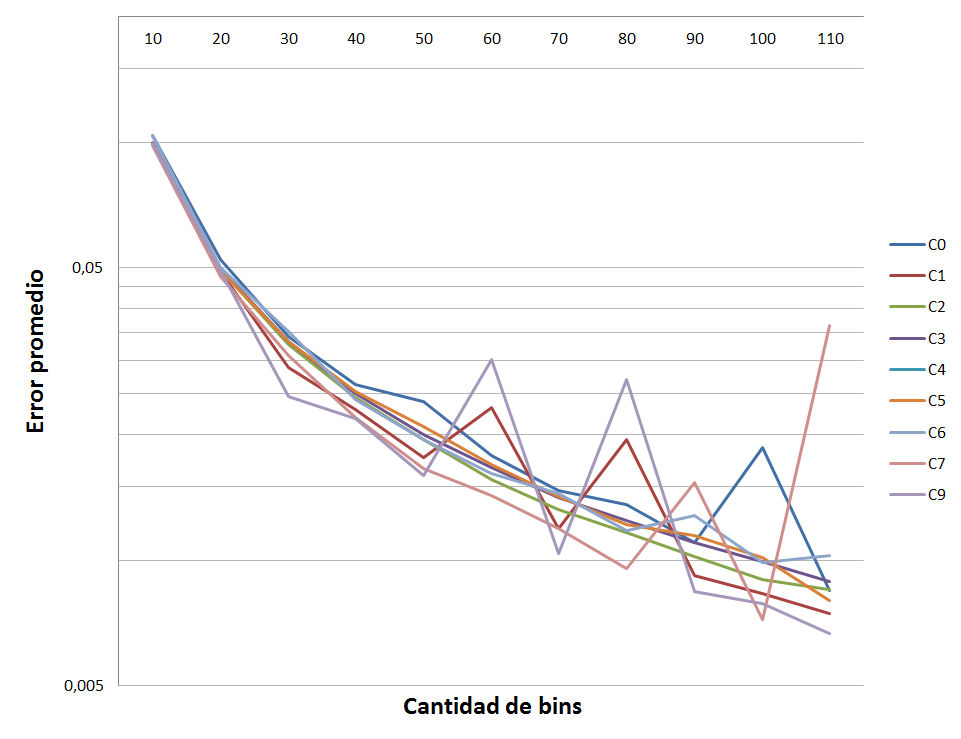
\includegraphics[scale=.60]{imagenes/variacion_parametro_y_columna_histo.png}
	    \caption{Error promedio en Histograma clasico para todas las columnas de la tabla brindada por la materia} 
	    \label{fig:variacion_parametro_y_columna_histo}
\end{figure}

\begin{figure}[H]
	    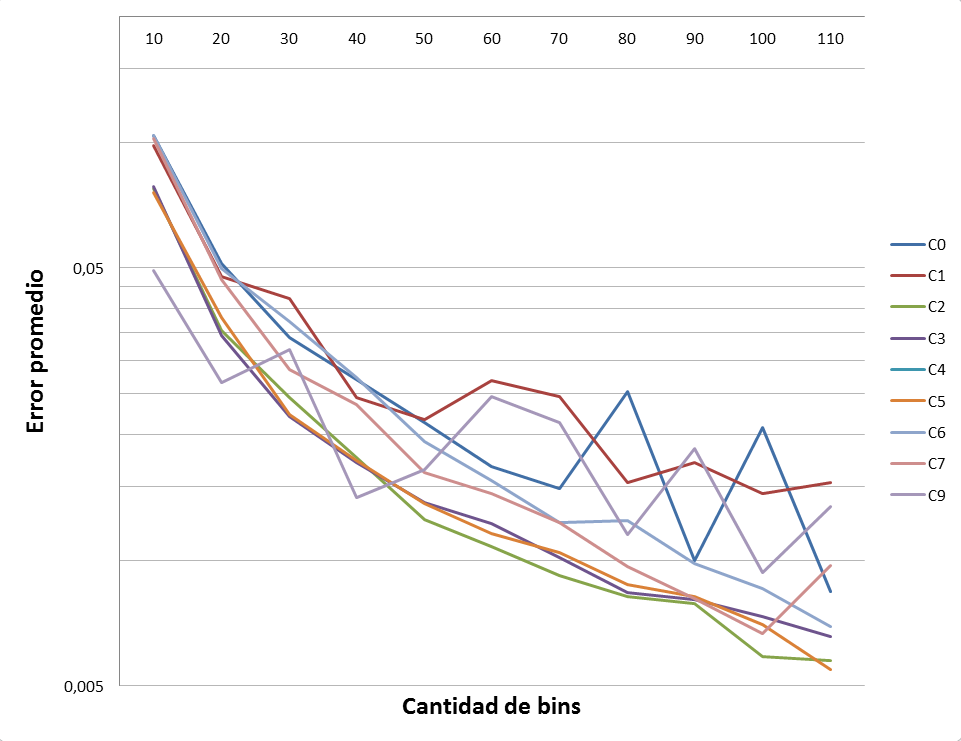
\includegraphics[scale=.60]{imagenes/variacion_parametro_y_columna_grupo.png}
	    \caption{Error promedio en Estimador del grupo para todas las columnas de la tabla brindada por la materia} 
	    \label{fig:variacion_parametro_y_columna_grupo}
\end{figure}

Adicionalmente, se puede ver en las figuras \ref{fig:variacion_parametro_y_columna_histo} y \ref{fig:variacion_parametro_y_columna_grupo} el mismo analisis realizado para Steps, pero esta ves para Histograma cl\'asico y el estimador echo por el grupo respectivamente. En estos graficos no se incluyo la columna C8, ya que la misma tiene datos que del 0 al 41, por lo que tienen un rango de 41, y para 50 buckets se tiene 1 bucket para cada valor, por lo que el error pasa a ser 0.

	Compar\'andolos con el gr\'afico de Steps, a primera vista se ve como en general Steps se comporta mejor considerando un valor del par\'ametro fijo. 
	
	A diferencia del de steps, el histograma cl\'asico no es tan independiente de la distribuci\'on de los datos, se puede ver como para las distintas columnas el error var\'ia bastante. 
	
	En cuanto al estimador del grupo, lo que se puede apreciar es que para algunas columnas, se comporta mejor que el Histograma cl\'asico, y dif\'icilmente se comporta mejor que Steps. Debido a lo analizado anteriormente, sabemos que el estimador del grupo tenia una mejor performance sobre el cl\'asico solo en las distribuciones normales, y en las uniformes los errores no variaban mucho entre uno y otro. Las columnas donde la performance es mejor que en el histograma, son las C2, C3 y C5. En el anexo a este informe, en la carpeta "/tests/Determinar Distribuciones" se encuentran los gr\'aficos de las columnas mencionadas. No fueron incluidos en este informe, debido a que eran demasiados y nos iban a quedar demasiados gr\'aficos. Tambien se encuentran graficadas las distribuciones de las columnas C1 y C9, que son las que obtuvieron errores mayores.
	
	En esos gr\'aficos, se puede ver como las distribuciones de esas columnas C2, C3 y C5 son todas normales, y C1 y C9 son de otra distribucion muy distinta, que no es normal ni uniforme, por lo que se puede comprobar que nuestro an\'alisis previo, en donde nuestro estimador se comportaba mejor en distribuciones normales, es correcto.
	